\subsection{Experimental Setup}
- describe i135
- describe benchmark set
- 900 seconds per instance

\subsection{Improvements to CrowdHTN}
- putting numbers to memory savings and how many nodes we save from instantiation (also saves our loop detection!)
- percentage of search nodes saved by not representing search nodes beginning with an action
- percentage of world states saved by sharing them between nodes

\subsection{Search Algorithms}
In section \ref{improv: search algorithms} we presented four search algorithms that we implemented for CrowdHTN. Those algorithms are random DFS, heuristic DFS, A-star like and BFS. We have tested all four algorithms on our test instance set using 4 PEs and a local bloom filter without restarts for loop detection. The results of this test are visualized in figure \ref{figure: algorithm eval}, a summary of coverage and IPC score is presented in table \ref{table: algorithm eval}. \\
Overall, random DFS performed best, followed by heuristic DFS, A-star like search and finally BFS with our best algorithm, random DFS, solving almost twice as many instances and having twice the IPC score of our worst algorithm, BFS. Additionally, we observe a hit-or-miss behavior in both our DFS implementations where plans are either found almost immediately or not at all. Out of the 50 instances solved by random DFS, only 18 were solved in more than 1 and out of these 18 only 9 were solved in more than 10 seconds. 

For both random and heuristic DFS, we see a hit-or-miss characteristic in our planner.

- our heuristic is just not that good
- the more we behave like BFS, the worse it gets
	- A-star gives a clear in between of BFS and our heuristic search
- BFS reduces the hit-or-miss nature of our search
\begin{figure}
	\caption{Plotting the number of solved instances per runtime for CrowdHTN using DFS, heuristic DFS, A-star like search and BFS}
	\label{figure: algorithm eval}
	\centering
	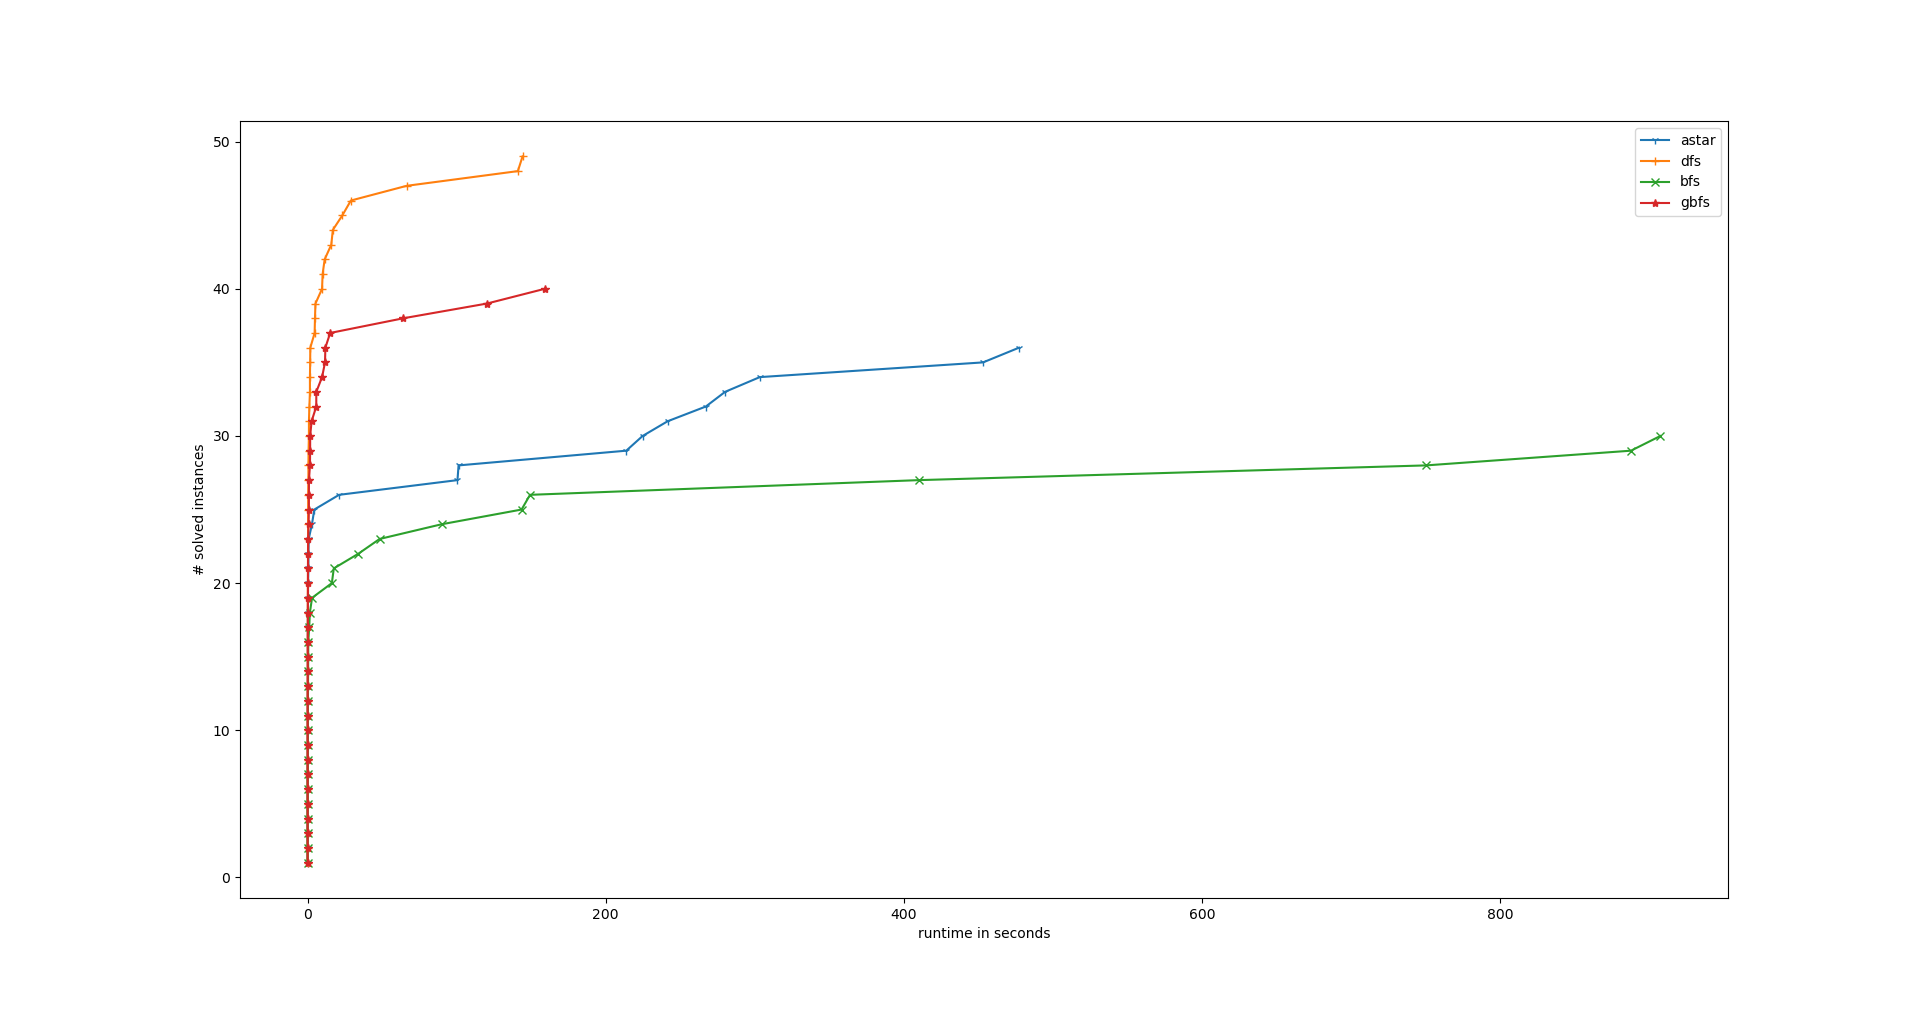
\includegraphics[width=\textwidth]{images/prelim/algorithms.png}
\end{figure}
\begin{table}
	\caption{Coverage and IPC score of our search algorithms using 4 PEs and a local bloom filter}
	\label{table: algorithm eval}
	\centering
	\begin{tabular}{| r | r | r |}
		\hline
		Algorithm 		& Solved Instances & IPC Score \\
		\hline
		Random DFS 		& 50	& 43.09 \\
		Heuristic DFS 	& 40	& 35.6	\\
		A-star like 	& 36	& 27.13 \\
		BFS 			& 30	& 21.87	\\
		\hline
	\end{tabular}
\end{table}

- comparison of search algorithms
- show just how bad BFS is? (branching factor + minimum layer through Lilotane)

\subsection{Scalability}
- show scaling on a nice instance

\subsection{Loop Detection}
- general loop detection:
- loop hit rate
- global loop hit rate
- performance of hash set vs bloom filter

\subsection{Probabilistic Restarts}
- test the probabilistic restarts
- with 900 seconds we expect $\sum_{t=1}^{899} \frac{1}{t} \approx 7.38$ restarts per run


\subsection{Global Loop Detection}
- test the global loop detection

\subsection{Malleable CrowdHTN}
- test the malleability

\subsection{Conclusion}
